\subsection{Algorithm for the simulation} \label{sec:detailed-algorithm}
	\begin{enumerate}
		\item \textbf{Input constants:} declare ${\mu}_{1}$, ${\mu}_{2}$, $l$, $\sigma$.
		
		\item \textbf{Input files:} read radius and meniscus distribution.
		
		\item \textbf{Random radius:} add very small random values to the radius distribution, so that there is an unique way of distributing fluids into the tubes.
		
		\item \textbf{Create pressure matrix:} create a 0 filled augmented matrix $M_{ij}$ of $n$ rows and $n + 1$ columns, where $n$ is the number of nodes in our system, this matrix will be solved to find the pressures in each node.
		
		\item \textbf{Set time:} set the physical time of our simulation $t = 0$.
		\item \textbf{Main loop:} until a certain saturation $S$ is reached in a given region, or for a fixed number of frames:
		\begin{enumerate}
			\item \textbf{Generate linear equations:} iterate for every $N_i$, $1 \le i \le n$:
			
			\begin{enumerate}
				\item \textbf{Generate connections:} the list of nodes $N_j$ and tubes $b_{ij}$, which are connected to $N_i$.
				
				\item \textbf{Iterate connections:} for each node $N_j$ connected to $N_i$:
				
				\begin{enumerate}
					\item $R_{ij}$ is obtained from radius distribution. Calculate $M_{ij}$ and $s_{ij}$ from current meniscus configuration of $b_{ij}$.
					
					\item Using $R_{ij}$, $M_{ij}$, $s_{ij}$, and other constants, calculate $A_{ij}$ and $B_{ij}$ according to equations \ref{eq:flow-rate-aij} and \ref{eq:flow-rate-bij}.
					
					\item Perform the following modifications to $M_{ij}$:
					
					$M_{ii} = M_{ii} + A_{ii}$
					
					$M_{ij} = M_{ij} - A_{ij}$
					
					$M_{i,n + 1} = M_{i,n + 1} - B_{ij}$
				\end{enumerate}
			\end{enumerate}
			
			\item \textbf{Calculate pressures:} solve $M_{ij}$. Gaussian-elimination was used for the results of simulations shown in this article.
			
			\item \textbf{Calculate velocity:} from the pressures calculated in each node, determine the velocity in each tube using equation \ref{eq:velocity-from-pressures}.
			
			\item \textbf{Calculate time step:} the time step for integration $\Delta t = min(\Delta t_{ij})$, here $\Delta t_{ij} = c_{t} min(l/v_{ij})$ for each tube $b_{ij}$. $c_{t} = 0.1$ was used for the simulations.
			
			\item \textbf{Calculate volume displacement}, the volume displaced in each tube is determined by, $V_{ij} = v_{ij} \Delta t$.
			
			\item \textbf{Store distribution:} iterate through each tube, and store how much of which fluid enters into the node towards which there is positive velocity.
			
			\item \textbf{Integration:} iterate through all the nodes, and for each node $N_i$: 
			
			\begin{enumerate}
				\item \textbf{List outflow tubes:} determine which tubes take away fluid from $N_i$.
				
				\item \textbf{Distribute} the wetting and non-wetting fluids according to the algorithm described in \ref{sec:multi-phase-flow}.
				
				\item \textbf{Recombine} when a tube has more than 2 menisci, according to \ref{sec:recombination-details}.
			\end{enumerate}
				
			\item \textbf{Picture:} save a picture of the current configuration.
			
			\item \textbf{Update saturation:} calculate the new saturation $S$.
			
			\item \textbf{Update time:} $t = t + \Delta t$.
			
			\item \textbf{Add plot point:} add $(t, S)$ to the plot.
		\end{enumerate}
		
		\item \textbf{Video:} a video file is generated from the pictures.	
	\end{enumerate}

		
\subsection{Modeling simple filtration: open boundaries} \label{sec:model-filtration}
	In a system with closed boundaries, no fluid can enter or leave the system. For the whole system, we have:
	
	\begin{equation}
		\frac{\partial S}{\partial t} = 0
	\end{equation}
	
	In a system with open boundaries, there is at least one node, into which fluid is externally added, and at least one node through which fluid leaves.
	
	Figure \ref{fig:simple-5-nodes} is an example of a system with open boundaries. We use open boundaries to test filtration. The nodes though which any amount of fluid can enter or leave is maintained at constant pressure.
	
	\begin{figure}[H]
		\centering
		\begin{subfigure}{0.47\textwidth}
			\centering
			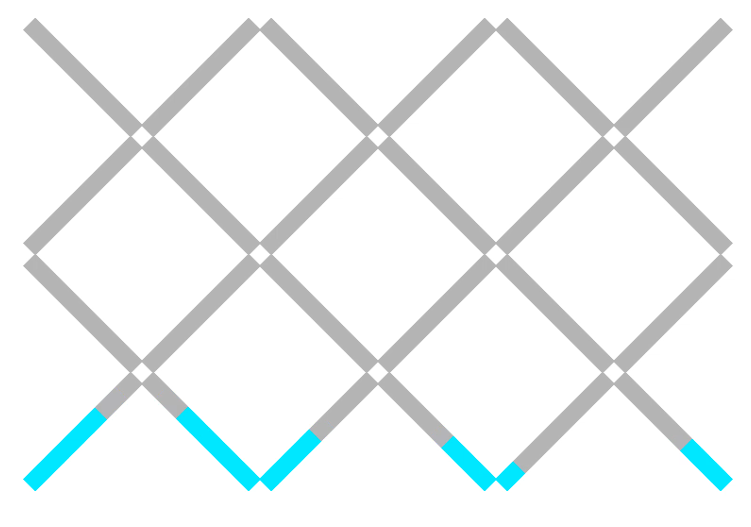
\includegraphics[width=\textwidth]{fig_initial-fill-distribution}
			\caption{Initial, wetting fluid confined to the bottom.}
			\label{fig:plot-sat-vs-time-disp-one}
		\end{subfigure}
		\begin{subfigure}{0.47\textwidth}
			\centering
			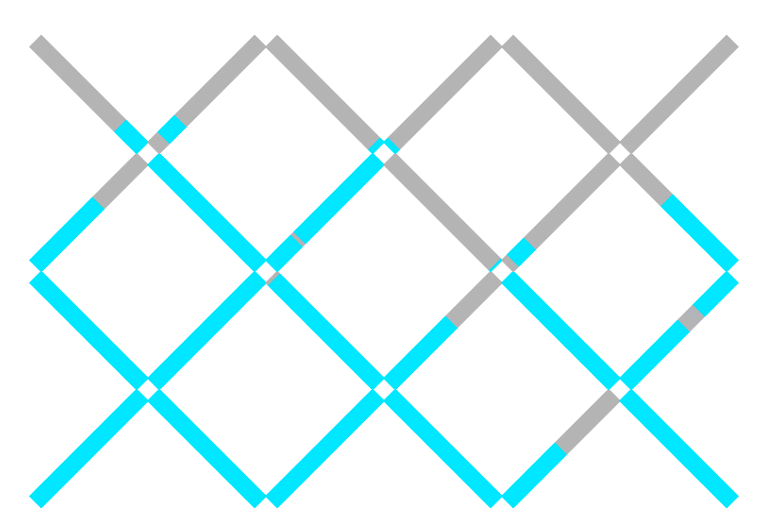
\includegraphics[width=\textwidth]{fig_final-fill-distribution}
			\caption{Wetting fluid invading due to external pressure.}
			\label{fig:plot-sat-vs-time-disp-two}
		\end{subfigure}
		\caption{Filtration with open boundaries.}
	\end{figure}
		
	Figure \ref{fig:plot-sat-vs-time-disp-one} consists of radius different thickness. A higher pressure is fixed for all nodes in the bottom layer, while a low pressure is fixed for the top row.

	
\subsection{Solution for closed boundaries} \label{sec:closed-boundary-triangle}

	In an open system, the matrix is of the form \ref{eq:matrix-open-sys-5-nodes}, and an unique solution always exists. However we will now show that the set of linear equations for a system with closed boundaries has infinitely many solutions.

	\begin{figure}[H]
		\centering
		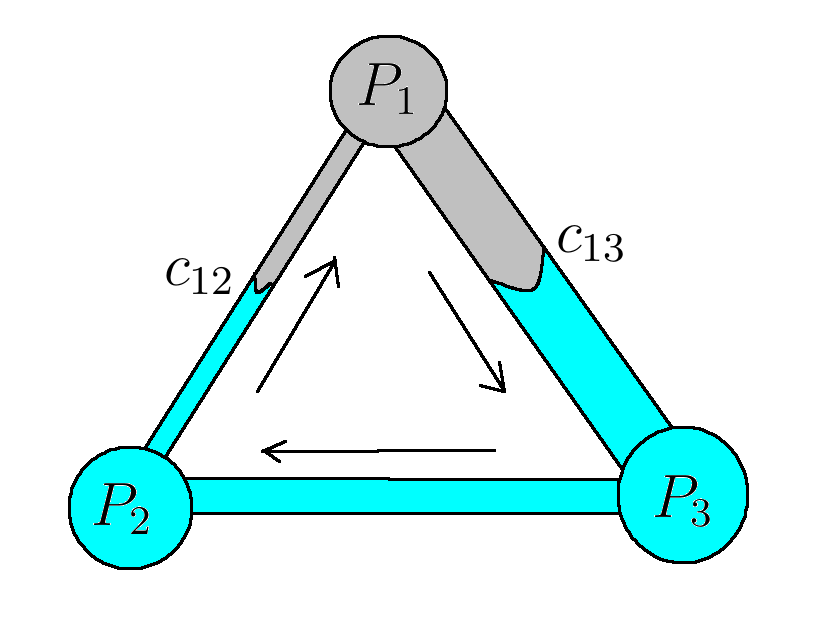
\includegraphics[height=4cm]{fig_zero-linearequation}
		\caption{Infinitely many solutions for a system with 3 nodes.}
		\label{fig:zero-la-triangle}
	\end{figure}
	
	The flow rates for $N_{1}$, according to equation \ref{eq:flow-rate-simple-coeff}:
	\begin{equation}
		Q_{12} = A_{12}(P_1 - P_2) + B_{12}
	\end{equation}
	
	\begin{equation}
		Q_{13} = A_{13}(P_1 - P_3) + B_{13}
	\end{equation}
	
	Due to conservation of volume:
	\begin{equation}
		Q_{12} + Q_{13} = 0
	\end{equation}
	
	So, we obtain:
	\begin{equation}
		(A_{12} + A_{13})P_1 - A_{12}P_2 - A_{13}P_3 = -B_{12} - B_{13}
	\end{equation}
	
	Applying the same for $N_2$ and $N_3$, we obtain the augmented matrix:
	\begin{equation}
		\begin{pmatrix}
			(A_{12} + A_{13}) & -A_{12} & -A_{13} & -B_{12} - B_{13} \\
			-A_{21} & (A_{21} + A_{23}) & -A_{23} & -B_{21} - B_{23} \\
			-A_{31} & -A_{32} & (A_{31} + A_{32}) & -B_{31} - B_{32} \\
		\end{pmatrix}
	\end{equation}
	
	From equation \label{eq:symmetry-of-b}, we have $B_{ij} = -B_{ji}$. So, the sum of all columns are zeros.
		
	After applying $R_3 = R_3 + R_1 + R_2$ to the matrix:
	
	\begin{equation}
		\begin{pmatrix}
			(A_{12} + A_{13}) & -A_{12} & -A_{13} & -B_{12} - B_{13} \\
			-A_{21} & (A_{21} + A_{23}) & -A_{23} & -B_{21} - B_{23} \\
			0 & 0 & 0 & 0 \\
		\end{pmatrix}
	\end{equation}
	
	We obtain a zero row. This problem is solved by adding a constant $a$ to one of the column of the matrix for every row. 
	\begin{equation}
		\begin{pmatrix}
			(A_{12} + A_{13}) & -A_{12} & -A_{13} + a & -B_{12} - B_{13} \\
			-A_{21} & (A_{21} + A_{23}) & -A_{23} + a & -B_{21} - B_{23} \\
			-A_{31} & -A_{32} & (A_{31} + A_{32}) + a & -B_{31} - B_{32} \\
		\end{pmatrix}
	\end{equation}
	
	This is the general case, when we have an arbitrary configuration of capillary pressures. In figure \ref{fig:zero-la-triangle}, $B_{21} = c_{12}, B_{13} = -c_{13}, B_{32} = 0$. Now, after $R_3 = R_3 + R_1 + R_2$:
	\begin{equation}
		\begin{pmatrix}
			(A_{12} + A_{13}) & -A_{12} & -A_{13} + a & -B_{12} - B_{13} \\
			-A_{21} & (A_{21} + A_{23}) & -A_{23} + a & -B_{21} - B_{23} \\
			0 & 0 & 3a & 0 \\
		\end{pmatrix}
	\end{equation}
	
	\begin{equation}
		3aP_3 = 0
	\end{equation}
	
	The solution exists only if $P_3 = 0$. This is point of zero pressure. In our simulation, the center was chosen to be the point of zero pressure. Changing this point does not change the flow rates or the nature of flows.

\subsection{Example of meniscus reaching a node: closed boundary} \label{sec:example-meniscus-in-node}
	\begin{figure}[H]
		\centering
		
		\begin{subfigure}{0.42\textwidth}
			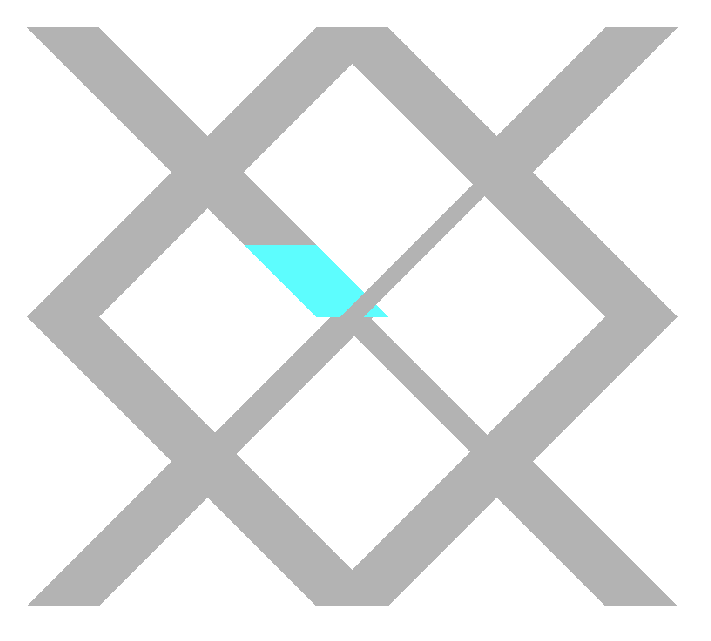
\includegraphics[width=\textwidth]{fig_test_dist_th01}
			\caption{Showing radius thickness}
		\end{subfigure}
		\hfill
		\begin{subfigure}{0.40\textwidth}
			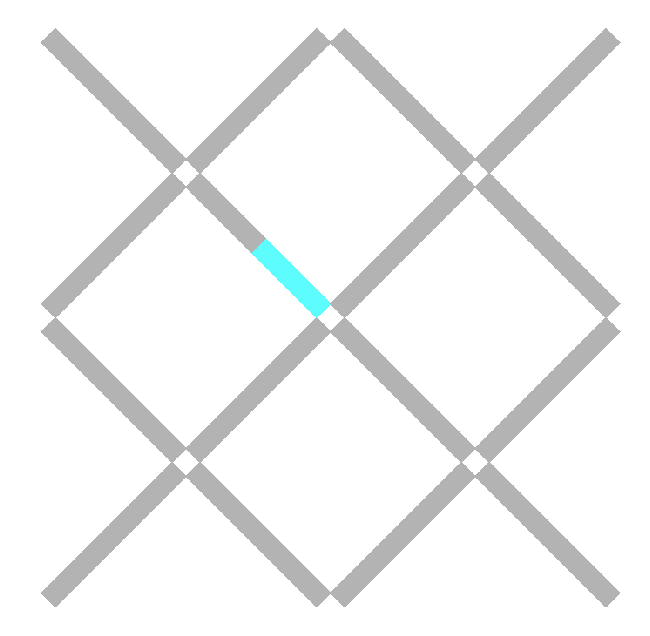
\includegraphics[width=\textwidth]{fig_test_dist_tn01}
			\caption{Without showing thickness}
		\end{subfigure}
		
		\caption{A meniscus just reached a node.}
	\end{figure}
	
	The tube where the cyan fluid is initially located is the thickest. After reaching the node, an additional 3 menisci are created very close to the node. Since the new tubes are all thinner than the initial. The capillary force from the new tubes is higher.
	
	\begin{figure}[H]
		\centering
		
		\begin{subfigure}{0.42\textwidth}
			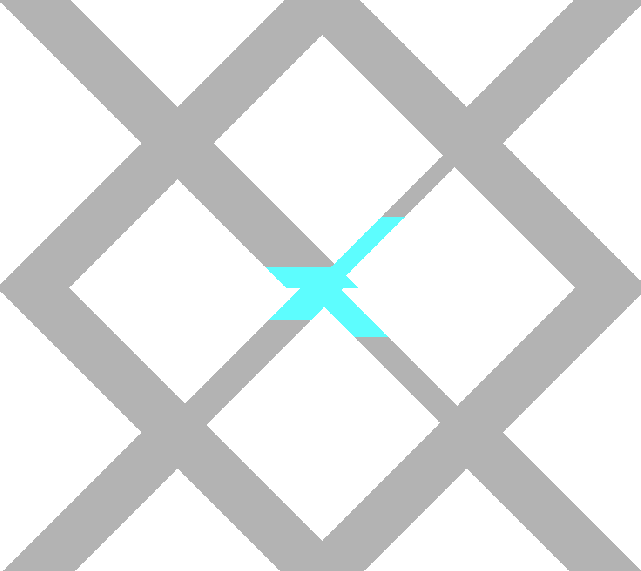
\includegraphics[width=\textwidth]{fig_test_dist_th04}
			\caption{Showing radius thickness}
		\end{subfigure}
		\hfill
		\begin{subfigure}{0.40\textwidth}
			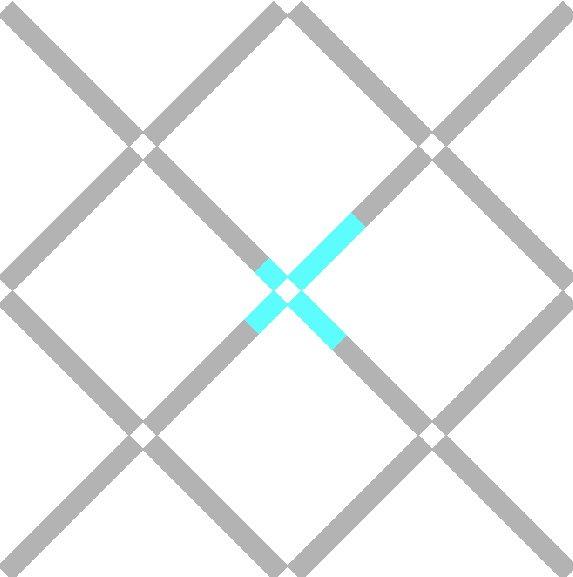
\includegraphics[width=\textwidth]{fig_test_dist_tn04}
			\caption{Without showing thickness}
		\end{subfigure}
		
		\caption{Cyan fluid being pulled by thinner tubes.}
	\end{figure}
	
	The thinnest tube pulls the cyan fluid away from the node the most, due to higher capillary pressure.
	
	
